\documentclass[tikz,border=6pt]{standalone}
\usepackage[utf8]{inputenc}
\usepackage[T1]{fontenc}
\usepackage{tikz}
\begin{document}
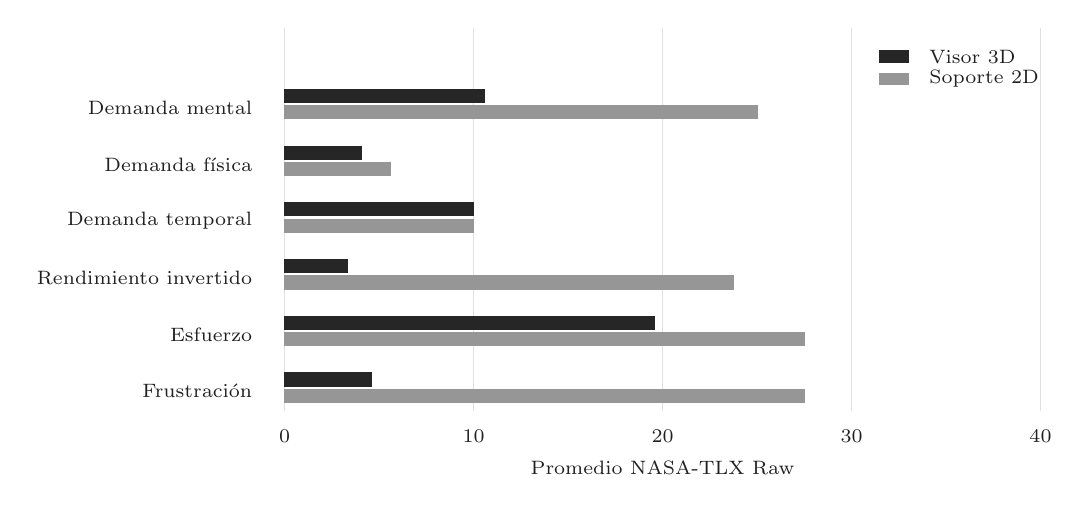
\begin{tikzpicture}[x=0.24cm,y=0.72cm,font=\sffamily]
  \definecolor{ink}{RGB}{32,32,32}
  \definecolor{soft}{RGB}{224,224,224}
  \definecolor{barA}{RGB}{38,38,38}
  \definecolor{barB}{RGB}{150,150,150}

  \foreach \x in {0,10,20,30,40} {
    \draw[soft, line width=0.4pt] (\x,-0.2) -- (\x,6.55);
    \node[ink, font=\scriptsize] at (\x,-0.65) {\x};
  }
  \node[ink, font=\scriptsize] at (20,-1.2) {Promedio NASA-TLX Raw};

  \foreach \label/\vA/\vB/\row in {
    {Demanda mental}/10.58/25.00/5,
    {Demanda física}/4.08/5.58/4,
    {Demanda temporal}/10.00/10.00/3,
    {Rendimiento invertido}/3.33/23.75/2,
    {Esfuerzo}/19.58/27.50/1,
    {Frustración}/4.58/27.50/0
  } {
    \node[anchor=east, ink, font=\scriptsize] at (-1.2,\row+0.15) {\label};
    \draw[fill=barB, draw=barB] (0,\row-0.05) rectangle (\vB,\row+0.18);
    \draw[fill=barA, draw=barA] (0,\row+0.24) rectangle (\vA,\row+0.47);
  }

  \draw[fill=barA, draw=barA] (31.5,5.95) rectangle (33.0,6.15);
  \node[anchor=west, ink, font=\scriptsize] at (33.6,6.05) {Visor 3D};
  \draw[fill=barB, draw=barB] (31.5,5.55) rectangle (33.0,5.75);
  \node[anchor=west, ink, font=\scriptsize] at (33.6,5.65) {Soporte 2D};
\end{tikzpicture}
\end{document}
